
\documentclass[a4paper,11pt]{article}
\usepackage{graphicx}
\usepackage{wrapfig}
\newcommand{\gtrsim}{\lower.5ex\hbox{$\; \buildrel > \over \sim \;$}}
\newcommand{\lesssim}{\lower.5ex\hbox{$\; \buildrel < \over \sim \;$}}
\newcommand\farcs{\mbox{$.\!\!^{\prime\prime}$}}% 
\pagestyle{empty}
\setlength{\topmargin}{-25mm}
\setlength{\textheight}{270mm}
\setlength{\textwidth}{180mm}
\setlength{\oddsidemargin}{-10mm}
\setlength{\evensidemargin}{-10mm}
\begin{document}

\begin {centering}
{\bf Measuring $H_0$ Through Detailed Modeling of 2 Quadruply Lensed Quasars} {\bf (PI: Rusu C. E.)}\\
 \end{centering}
 
\medskip

\noindent {\bf Abstract.} Using adaptive optics (AO) observations we aim to construct detailed mass models of two quadruply lensed quasars, for which our previous work has shown that high-resolution imaging is paramount. By modeling the extended emission from their quasar host galaxies, in conjunction with ongoing optical monitoring, we will use these two systems to improve the inference of $H_0$ via the time delay technique.

The recent tension between direct measurements of $H_{0}$ based on the distance ladder and that derived by the {\it Planck} team within the assumptions of a six-parameter flat $\Lambda$CDM model highlights the need for multiple independent techniques (Riess et al. 2016, ApJ, 826, 56, fig. 1). If the tension cannot be resolved by unknown systematics, it will force the rejection of the six-parameter model in favor of more complex alternatives (e.g., $w \ne -1$, variable effective number of relativistic neutrino species), leading to new physics. 

The time-delay technique (Refsdal 1964, MNRAS, 128, 307), applied to a moderate number of strongly lensed quasars, allows one to reach percent accuracy on $H_{0}$ (Suyu et al. 2013, ApJ, 766, 70). By measuring the time delay $\Delta t$ between pairs of lensed images, and accurately modeling the mass distribution of the lens galaxy, the time delay distance $D_{\Delta t}$ can be inferred. This quantity is primarily sensitive to $H_{0}$, with $D_{\Delta t} \propto H_{0}^{-1}$. The method is based on simple geometry and well-tested physics (i.e., general relativity) rather than complicated astrophysics (e.g., dust, evolution, etc.). Since each time-delay distance is independent, a sample of N time-delay lenses leads to a reduction in the statistical uncertainty by $\sqrt{\mathrm{N}}$. With measurements from just three time delay lenses (blue shaded area in fig. 1, right) we have already achieved 3.8\% precision on $H_{0}$ (Bonvin et al. 2017, MNRAS, 465, 4914). {\it With this proposal, we aim to to get to 2\% precision on $H_{0}$ (red shaded area)} from a total sample of nine quadruply lensed quasars. Quadruple lenses, as opposed to doubles, offer more mass modeling constraints and three time delays instead of one. Only two of our lenses lack the required high-resolution imaging to accurately measure the mass distribution of the lens galaxies.

 We have recently discovered our two targets from PanSTARRS+2MASS (Lucey et al. 2018, MNRAS, 476, 927; Rusu et al. 2018, arXiv:1803.07175). 2M1134-2103 at $z_{QSO}=2.77$ has a unique diamond-like configuration indicative of very large external shear. Existing data is insufficient to characterize the morphology of the highly blended lensing galaxy, but it suggests the influence of a nearby perturber (fig. 1, left). 2M1310-1714 at $z_\mathrm{QSO}=1.98$, $z_\mathrm{lens}=0.29$ has two lensing galaxy between which a rare 5th quasar image is predicted to exist, but has not been detected in the shallow, low-resolution available data. The brightness of the first system and the large image separation ($\sim7''$) of the second makes them ideal for monitoring (already in progress) to measure time delays.

{\bf Ancillary Science.} Both our source quasars are at $z\gtrsim2$, where only $\sim$ a dozen quasars have benefited from a study of the supermassive black hole - host galaxy relation (e.g., Ding et al. 2017, MNRAS, 472, 90). Our proposed observations, which are aimed at characterizing the hosts, will naturally add to this study.

{\bf Proposed Observations.} We propose a combined 4 hours of IRCS+AO188+LGS $K'$-band imaging observations of our two lenses. In the short term, we will use the data to investigate the mass distribution in these intriguing systems. In the long term, we will combine them with our seven existing systems with available ancillary data, in order to reach 2\% precision on $H_{0}$. As Chen et al. 2016 (MNRAS, 462, 3457) has shown, AO data is superior for this task to \textit{HST} data, and the point spread function can be reconstructed from the data itself, allowing to accurately characterize the host galaxies. 

\begin{minipage}{\textwidth}
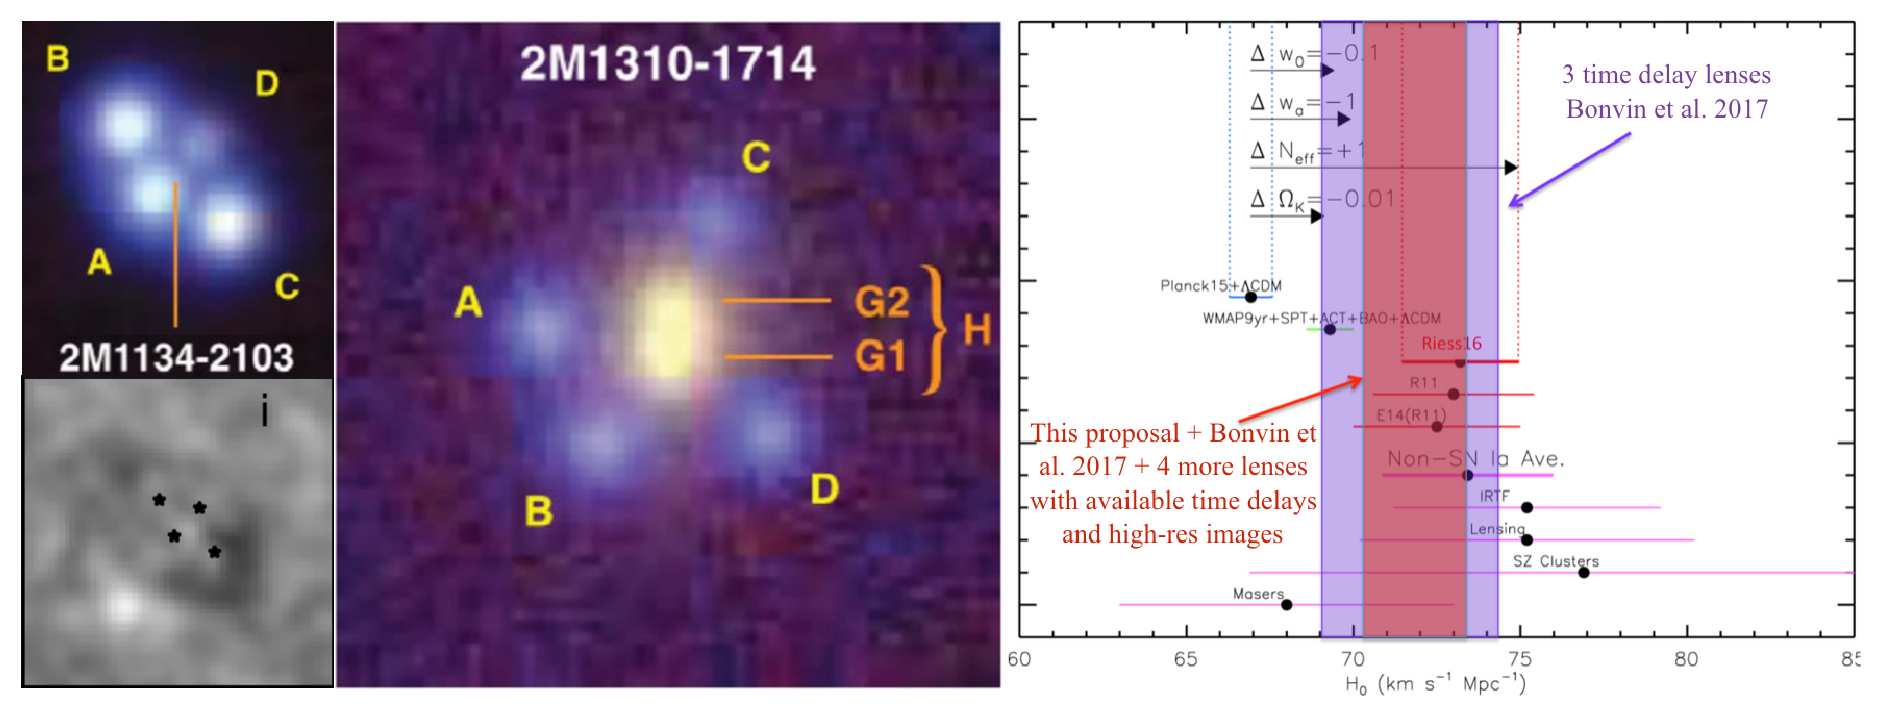
\includegraphics[width=0.95\hsize]{figure.eps}
\end{minipage}
Fig. 1: {\it Top left:} PanSTARRS image of 2M1134-2103 (Lucey et al. 2018). {\it Bottom left:} A nearby perturber may be responsible for the large shear (Rusu et al. 2018). {\it Center:} PanSTARRS image of 2M1310-1714 (Lucey et al. 2018). {\it Right:} Tension between measurements of $H_{0}$ from different probes in a $\Lambda$CDM cosmology, and expected improvement based on the proposed data (based on Riess et al. 2016).
  
\end{document}
